% !TeX program = lualatex
\documentclass[12pt, a4paper]{article}
\usepackage{fullpage}
\usepackage{subfiles}
\usepackage{fontspec}
\usepackage{libertine}
\usepackage{xcolor}
\usepackage{GotIn}
\usepackage{geometry}
\usepackage{multicol}
\usepackage{multicolrule}
\usepackage{graphicx}
\usepackage{enumitem}
\usepackage[autocompile]{gregoriotex}
\usepackage[latin,french]{babel}


\geometry{top=2cm, bottom=2cm}
\pagestyle{empty}

\definecolor{red}{HTML}{C70039}
% \input GoudyIn.fd
% \newcommand*\initfamily{\usefont{U}{GoudyIn}{xl}{n}}

\input Acorn.fd
\newcommand*\initfamily{\usefont{U}{Acorn}{xl}{n}}
% cette ligne ajoute de l'espace entre les portées
% \grechangedim{baselineskip}{60pt}{scalable}

\begin{document}
  \gresetlinecolor{gregoriocolor}

  \begin{titlepage}\centering
    \vspace*{\fill}\
    \huge Secondes Vêpres\\
    \smallskip
    \begin{Large}
      \textit{
        Fête de la Sainte Trinité\\
      }
    \end{Large}
    \medskip
    \large et\\
    \medskip
    \LARGE Salut du Saint-Sacrement\\
    \bigskip
    % \begin{figure}[h!]
    %   \centering
    %   
\includegraphics[width=7cm]{../ordinaires/logo.png}
    % \end{figure}
    \vspace*{\fill}
    \begin{figure}[h!]
      \centering
      
\includegraphics[width=7cm]{../ordinaires/logo.png}
    \end{figure}
    \centering \normalsize Paroisse Saint Roch\\
    \bigskip
    \begin{Large}
      \centering Ne pas emporter
    \end{Large}
  \end{titlepage}

  \newpage
  \vspace*{\fill}
    \begin{center}
      \normalsize\textit{
        Livret latin-français
      }
    \end{center}
  \newpage

  \begin{center}
    \textcolor{red}{\large{Ouverture.}}
  \end{center}

  % greillumination: remplace la première lettre, ici par une font ornementale
  \greillumination{\initfamily\fontsize{11mm}{11mm}\selectfont D}
  \gregorioscore{../ordinaires/vepres-deus_in_adjutorium}

  \begin{center}
    \small{
    \emph{
      Dieu, venez à mon aide ; Seigneur, hatez-vous de me secourir.\\
      Gloire au Père, au Fils et au Saint Esprit, comme il était au commencement, maintenant et toujour et dans les siècles des siècles. Allelúia\\
    }
  }
  \end{center}

  \newpage
  \normalsize

  % ===== DEBUT Antienne =========
  \gresetinitiallines{1}
  \greillumination{\initfamily\fontsize{11mm}{11mm}\selectfont G}
  \gregorioscore{antiennes/an--gloria_tibi_trinitas--solesmes_1961}
  \begin{center}
    \footnotesize{
      \textit{Gloire à vous, Trinité égale, Divinité une qui êtes avant tous les siècles, et maintenant et toujours. }
    }
  \end{center}
  % ===== FIN Antienne ===========

  % ===== DEBUT psaume ===========
  % gresetinitiallines : avec le parametre à 0, supprime l'ornement
  \begin{center}
    \large{Psaume 109.}\\
  \end{center}

  \gresetinitiallines{0}
  \gregorioscore{psaumes/psaume109-If}

  \begin{enumerate}[label=\textcolor{red}{\arabic*}]
    \setcounter{enumi}{1}
    \item Donec ponam in\textit{i}\textit{mí}\textit{cos} \textbf{tu}os,\textcolor{red}{~*} scabéllum pe\textit{dum} \textit{tu}\textbf{ó}rum.

    \item Virgam virtútis tuæ emíttet Dó\textit{mi}\textit{nus} \textit{ex} \textbf{Si}on:\textcolor{red}{~*} domináre in médio inimicó\textit{rum} \textit{tu}\textbf{ó}rum.

    \item Tecum princípium in die virtútis tuæ in splendó\textit{ri}\textit{bus} \textit{sanc}\textbf{tó}rum:\textcolor{red}{~*} ex útero ante lucíferum \textit{gé}\textit{nu}\textbf{i} te.

    \item Jurávit Dóminus, et non pœ\textit{ni}\textit{té}\textit{bit} \textbf{e}um:\textcolor{red}{~*} Tu es sacérdos in ætérnum secúndum órdi\textit{nem} \textit{Mel}\textbf{chí}sedech.

    \item Dóminus \textit{a} \textit{dex}\textit{tris} \textbf{tu}is,\textcolor{red}{~*} confrégit in die iræ \textit{su}\textit{æ} \textbf{re}ges.

    \item Judicábit in natiónibus, im\textit{plé}\textit{bit} \textit{ru}\textbf{í}nas:\textcolor{red}{~*} conquassábit cápita in ter\textit{ra} \textit{mul}\textbf{tó}rum.

    \item De torrénte \textit{in} \textit{vi}\textit{a} \textbf{bi}bet:\textcolor{red}{~*} proptérea exal\textit{tá}\textit{bit} \textbf{ca}put.

    \item Glória \textit{Pa}\textit{tri}, \textit{et} \textbf{Fí}\textbf{li}o,\textcolor{red}{~*} et Spirí\textit{tu}\textit{i} \textbf{Sanc}to.

    \item Sicut erat in princípio, \textit{et} \textit{nunc}, \textit{et} \textbf{sem}per,\textcolor{red}{~*} et in sǽcula sæcu\textit{ló}\textit{rum}. \textbf{A}men.
  \end{enumerate}
  %  Répetition de l'Antienne
  \grecommentary{\textit{Reprise de l'Antienne.}}
  \gabcsnippet{(c4) Gló(d!ewf)ri(d)a(d) (,) ti(d_c)bi(f_g) Trí(gf)ni(gh)tas(h) ae(h)quá(h_j)lis,(h'_) (,) u(h)na(gf) Dé(g)i(gh)tas,(h.) (;) et(h) an(h_j!kvJH'i)te(h') ó(h)mni(h)a(hg) saé(h)cu(gf)la,(g_[uh:l]h) (;) et(f) nunc,(ghg) et(fe) in(f) per(fgf')pé(d)tu(cd)um.(d.) (::)}

  \newpage
  \vspace*{\fill}\
  \begin{normalsize}
    \begin{center}
      \par \textit{Gloire à vous, Trinité égale, Divinité une qui êtes avant tous les siècles, et maintenant et toujours.}
      \medskip
      \begin{enumerate}[label=\textcolor{red}{\emph{\arabic*}}]
        \item \textit{Le Seigneur a dit à mon Seigneur : Asseyez-toi à ma droite, }
        \item \textit{Jusqu'à ce que je mette tes ennemis pour le marchepied de tes pieds.}
        \item \textit{L'Éternel enverra de Sion la verge de ta force: Domine au milieu de tes ennemis!}
        \item \textit{Ton peuple sera un peuple de franche volonté, au jour de ta puissance, en sainte magnificence. Du sein de l'aurore te viendra la rosée de ta jeunesse.}
        \item \textit{L'Éternel a juré, et il ne se repentira point: Tu es sacrificateur pour toujours, selon l'ordre de Melchisédec.}
        \item \textit{Le Seigneur, à ta droite, brisera les rois au jour de sa colère.}
        \item \textit{Il jugera parmi les nations, il remplira tout de corps morts, il brisera le chef d'un grand pays.}
        \item \textit{Il boira du torrent dans le chemin, c'est pourquoi il lèvera haut la tête.}
        \item \textit{Gloire au Père, au Fils, et au Saint Esprit, }
        \item \textit{Comme il était au commencement, maintenant et toujours, et dans les siècles des siècles. Amen. }
      \end{enumerate}
    \end{center}
  \end{normalsize}
  \vspace*{\fill}\
  \newpage

  % ===== DEBUT Antienne =========
  \gresetinitiallines{1}
  \greillumination{\initfamily\fontsize{11mm}{11mm}\selectfont L}
  \gregorioscore{antiennes/an--laus_et_perennis_gloria--solesmes_1961}
  \begin{center}
    \footnotesize{
      \textit{Louange et gloire éternelle soient à Dieu le Père, et au Fils, et en même temps au saint Paraclet, dans les siècles des siècles. }
    }
  \end{center}
  % ===== FIN Antienne ===========

  % ===== DEBUT psaume ===========
  % gresetinitiallines : avec le parametre à 0, supprime l'ornement
  \begin{center}
    \large{Psaume 110.}\\
  \end{center}

  \gresetinitiallines{0}
  \gregorioscore{psaumes/psaume110-IID}

  \begin{enumerate}[label=\textcolor{red}{\arabic*}]
    \setcounter{enumi}{1}
    \item Magna ópera \textbf{Dó}mini:\textcolor{red}{~*} exquisíta in omnes voluntá\textit{tes} \textbf{e}jus.

    \item Conféssio et magnificéntia opus \textbf{e}jus:\textcolor{red}{~*} et justítia ejus manet in sǽcu\textit{lum} \textbf{sǽ}culi.

    \item Memóriam fecit mirabílium suórum,\textcolor{red}{~†}  miséricors et miserátor \textbf{Dó}minus:\textcolor{red}{~*} escam dedit timén\textit{ti}\textbf{bus} se.

    \item Memor erit in sǽculum testaménti \textbf{su}i:\textcolor{red}{~*} virtútem óperum suórum annuntiábit pópu\textit{lo} \textbf{su}o:

    \item Ut det illis hereditátem \textbf{gén}tium:\textcolor{red}{~*} ópera mánuum ejus véritas, et \textit{ju}\textbf{dí}cium.

    \item Fidélia ómnia mandáta ejus:\textcolor{red}{~†}  confirmáta in sǽculum \textbf{sǽ}culi,\textcolor{red}{~*} facta in veritáte et æ\textit{qui}\textbf{tá}te.

    \item Redemptiónem misit pópulo \textbf{su}o:\textcolor{red}{~*} mandávit in ætérnum testamén\textit{tum} \textbf{su}um.

    \item Sanctum, et terríbile nomen \textbf{e}jus:\textcolor{red}{~*} inítium sapiéntiæ ti\textit{mor} \textbf{Dó}mini.

    \item Intelléctus bonus ómnibus faciéntibus \textbf{e}um:\textcolor{red}{~*} laudátio ejus manet in sǽcu\textit{lum} \textbf{sǽ}culi.

    \item Glória Patri, et \textbf{Fí}lio,\textcolor{red}{~*} et Spirítu\textit{i} \textbf{Sanc}to.

    \item Sicut erat in princípio, et nunc, et \textbf{sem}per,\textcolor{red}{~*} et in sǽcula sæculó\textit{rum}. \textbf{A}men.
  \end{enumerate}
  %  Répetition de l'Antienne
  \grecommentary{\textit{Reprise de l'Antienne.}}
  \gabcsnippet{(f3) Laus(ff) et(e) per(f')én(h)nis(hih') gló(f)ri(ef)a(f.) (,) De(fh)o(f) Pa(fe)tri,(f') et(h) Fí(h)li(fe)o,(e.) (;) san(ef~)cto(f) si(fe)mul(f') Pa(h)rá(i')cli(h)to,(h'_) (,) in(h) saé(i)cu(hg)la(h') sae(i)cu(hg)ló(f.)rum.(f.) (::)}

  \newpage
  \vspace*{\fill}\
  \begin{normalsize}
    \begin{center}
      \par \textit{Louange et gloire éternelle soient à Dieu le Père, et au Fils, et en même temps au saint Paraclet, dans les siècles des siècles.}
      \medskip
      \begin{enumerate}[label=\textcolor{red}{\emph{\arabic*}}]
        \item \textit{De tout cœur je rendrai grâce au Seigneur dans l'assemblée, parmi les justes.}
        \item \textit{Grandes sont les œuvres du Seigneur ; tous ceux qui les aiment s'en instruisent.}
        \item \textit{Noblesse et beauté dans ses actions : à jamais se maintiendra sa justice.}
        \item \textit{De ses merveilles il a laissé un mémorial ; le Seigneur est tendresse et pitié, il a donné des vivres à ses fidèles,}
        \item \textit{Gardant toujours mémoire de son
        alliance, il a montré sa force à son peuple.}
        \item \textit{Lui donnant le domaine des nations. Justesse et sûreté les œuvres de ses mains.}
        \item \textit{Sécurité, toutes ses lois, établies pour toujours et à jamais, accomplies avec droiture et sûreté ! }
        \item \textit{Il apporte la délivrance à son peuple ; son alliance est promulguée pour toujours.}
        \item \textit{Saint, redoutable est son nom, la sagesse commence avec la crainte du Seigneur.}
        \item \textit{Qui accomplit sa volonté en est éclairé. A jamais se maintiendra sa louange.}
        \item \textit{Gloire au Père, au Fils, et au Saint Esprit, }
        \item \textit{Comme il était au commencement, maintenant et toujours, et dans les siècles des siècles. Amen. }
      \end{enumerate}
    \end{center}
  \end{normalsize}
  \vspace*{\fill}\
  \newpage

  % ===== DEBUT Antienne =========
  \gresetinitiallines{1}
  \greillumination{\initfamily\fontsize{11mm}{11mm}\selectfont G}
  \gregorioscore{antiennes/an--gloria_laudis_resonet--solesmes_1961}
  \begin{center}
    \footnotesize{
      \textit{Qu’une louange résonne sur les lèvres de tous à la gloire du Père et du Fils qu’il engendre, et qu’une même louange éternelle s’adresse au Saint-Esprit. }
    }
  \end{center}
  % ===== FIN Antienne ===========

  % ===== DEBUT psaume ===========
  % gresetinitiallines : avec le parametre à 0, supprime l'ornement
  \begin{center}
    \large{Psaume 111.}\\
  \end{center}

  \gresetinitiallines{0}
  \gregorioscore{psaumes/psaume111-IIIa2}

  \begin{enumerate}[label=\textcolor{red}{\arabic*}]
    \setcounter{enumi}{1}
    \item Potens in terra erit \textbf{se}men \textbf{e}jus:\textcolor{red}{~*} generátio rectórum be\textit{ne}\textit{di}\textbf{cé}tur.

    \item Glória, et divítiæ in \textbf{do}mo \textbf{e}jus:\textcolor{red}{~*} et justítia ejus manet in sǽ\textit{cu}\textit{lum} \textbf{sǽ}culi.

    \item Exórtum est in ténebris \textbf{lu}men \textbf{rec}tis:\textcolor{red}{~*} miséricors, et miserá\textit{tor}, \textit{et} \textbf{jus}tus.

    \item Jucúndus homo qui miserétur et cómmodat,\textcolor{red}{~†}  dispónet sermónes suos \textbf{in} ju\textbf{dí}\textbf{ci}o:\textcolor{red}{~*} quia in ætérnum non \textit{com}\textit{mo}\textbf{vé}bitur.

    \item In memória ætérna \textbf{e}rit \textbf{jus}tus:\textcolor{red}{~*} ab auditióne mala \textit{non} \textit{ti}\textbf{mé}bit.

    \item Parátum cor ejus speráre in Dómino,\textcolor{red}{~†}  confirmátum \textbf{est} cor \textbf{e}jus:\textcolor{red}{~*} non commovébitur donec despíciat ini\textit{mí}\textit{cos} \textbf{su}os.

    \item Dispérsit, dedit paupéribus:\textcolor{red}{~†}  justítia ejus manet in \textbf{sǽ}culum \textbf{sǽ}\textbf{cu}li,\textcolor{red}{~*} cornu ejus exaltábi\textit{tur} \textit{in} \textbf{gló}ria.

    \item Peccátor vidébit, et irascétur,\textcolor{red}{~†}  déntibus suis fremet \textbf{et} ta\textbf{bé}scet:\textcolor{red}{~*} desidérium peccató\textit{rum} \textit{per}\textbf{í}bit.

    \item Glória \textbf{Pa}tri, et \textbf{Fí}\textbf{li}o,\textcolor{red}{~*} et Spirí\textit{tu}\textit{i} \textbf{Sanc}to.

    \item Sicut erat in princípio, et \textbf{nunc}, et \textbf{sem}per,\textcolor{red}{~*} et in sǽcula sæcu\textit{ló}\textit{rum}. \textbf{A}men.
  \end{enumerate}
  %  Répetition de l'Antienne
  \grecommentary{\textit{Reprise de l'Antienne.}}
  \gabcsnippet{(c4) Gló(e_[oh:h]d)ri(g)a(hj) lau(i_[uh:l]j)dis(j.) (,) ré(ji)so(h)net(i) in(jk) o(k)re(ji) ó(hi)mni(hg)um,(g.) (;) Pa(g_[uh:l]h)tri,(g) ge(e)ni(ed)taé(g)que(hj) Pro(i_[uh:l]j)li,(j.) (;) Spi(j)rí(ji)tu(h)i(i_[uh:l]j) San(k)cto(ji) pá(hi)ri(hg)ter(g'_[oh:h]) (,) re(g)súl(hi~)tet(h) lau(gf~)de(g) per(ghg)én(e.)ni.(e.) (::)}

  \newpage
  \vspace*{\fill}\
  \begin{normalsize}
    \begin{center}
      \par \textit{Qu’une louange résonne sur les lèvres de tous à la gloire du Père et du Fils qu’il engendre, et qu’une même louange éternelle s’adresse au Saint-Esprit.}
      \medskip
      \begin{enumerate}[label=\textcolor{red}{\emph{\arabic*}}]
        \item \textit{Heureux l’homme qui craint le Seigneur, qui aime entièrement sa volonté !}
        \item \textit{Sa lignée sera puissante sur la terre ; la
        race des justes est bénie.}
        \item \textit{Les richesses affluent dans sa maison : à
        jamais se maintiendra sa justice.}
        \item \textit{Lumière des cœurs droits, il s'est levé
        dans les ténèbres, l’homme de justice, de
        tendresse et de pitié.}
        \item \textit{L'homme de bien a pitié, il partage ; il
        mène ses affaires avec droiture, cet
        homme jamais ne tombera ;}
        \item \textit{Toujours on fera mémoire du juste, il ne
        craint pas l'annonce d'un malheur :}
        \item \textit{Le cœur ferme, il s'appuie sur le
        Seigneur. Son cœur est confiant, il ne
        craint pas : il verra ce que valaient ses
        oppresseurs.}
        \item \textit{A pleines mains, il donne au pauvre ; à
        jamais se maintiendra sa justice, sa
        puissance grandira, et sa gloire !}
        \item \textit{L'impie le voit et s'irrite ; il grince des
        dents et se détruit. L'ambition des impies
        se perdra.}
        \item \textit{Gloire au Père, au Fils, et au Saint Esprit, }
        \item \textit{Comme il était au commencement, maintenant et toujours, et dans les siècles des siècles. Amen. }
      \end{enumerate}
    \end{center}
  \end{normalsize}
  \vspace*{\fill}\
  \newpage

  % ===== DEBUT Antienne =========
  \gresetinitiallines{1}
  \greillumination{\initfamily\fontsize{11mm}{11mm}\selectfont L}
  \gregorioscore{antiennes/an--laus_deo_patri--solesmes_1961}
  \begin{center}
    \footnotesize{
      \textit{Louange à Dieu le Père et au Fils qui lui est égal, et que notre bouche, ô Esprit-Saint, fasse toujours retentir votre louange avec un constant amour. }
    }
  \end{center}
  % ===== FIN Antienne ===========

  % ===== DEBUT psaume ===========
  % gresetinitiallines : avec le parametre à 0, supprime l'ornement
  \begin{center}
    \large{Psaume 112.}\\
  \end{center}

  \gresetinitiallines{0}
  \gregorioscore{psaumes/psaume112-IVE}

  \begin{enumerate}[label=\textcolor{red}{\arabic*}]
    \setcounter{enumi}{1}
    \item Sit nomen Dómini \textit{be}\textit{ne}\textbf{díc}tum,\textcolor{red}{~*} ex hoc nunc, et \textit{us}\textit{que} \textit{in} \textbf{sǽ}\textbf{cu}lum.

    \item A solis ortu usque \textit{ad} \textit{oc}\textbf{cá}sum,\textcolor{red}{~*} laudábi\textit{le} \textit{no}\textit{men} \textbf{Dó}\textbf{mi}ni.

    \item Excélsus super omnes \textit{gen}\textit{tes} \textbf{Dó}minus,\textcolor{red}{~*} et super cælos \textit{gló}\textit{ri}\textit{a} \textbf{e}jus.

    \item Quis sicut Dóminus, Deus noster, qui in \textit{al}\textit{tis} \textbf{há}bitat,\textcolor{red}{~*} et humília réspicit in cæ\textit{lo} \textit{et} \textit{in} \textbf{ter}ra?

    \item Súscitans a \textit{ter}\textit{ra} \textbf{ín}opem,\textcolor{red}{~*} et de stércore \textit{é}\textit{ri}\textit{gens} \textbf{páu}\textbf{pe}rem:

    \item Ut cóllocet eum \textit{cum} \textit{prin}\textbf{cí}pibus,\textcolor{red}{~*} cum princípibus \textit{pó}\textit{pu}\textit{li} \textbf{su}i.

    \item Qui habitáre facit stéri\textit{lem} \textit{in} \textbf{do}mo,\textcolor{red}{~*} matrem fili\textit{ó}\textit{rum} \textit{læ}\textbf{tán}tem.

    \item Glória Pa\textit{tri}, \textit{et} \textbf{Fí}lio,\textcolor{red}{~*} et Spi\textit{rí}\textit{tu}\textit{i} \textbf{Sanc}to.

    \item Sicut erat in princípio, et \textit{nunc}, \textit{et} \textbf{sem}per,\textcolor{red}{~*} et in sǽcula sæ\textit{cu}\textit{ló}\textit{rum}. \textbf{A}men.
  \end{enumerate}
  %  Répetition de l'Antienne
  \grecommentary{\textit{Reprise de l'Antienne.}}
  \gabcsnippet{(c4) Laus(ev_[oh:h]ddf) De(dc)o(de) Pa(e)tri,(e'_[oh:h]) (,) pa(e)ri(dc)lí(d)que(de) Pro(e)li,(e.) (;) et(e') ti(g)bi(gh) San(h_i)cte(h'_) (,) stú(h)di(g')o(h) per(ih)én(gg)ni(e_[uh:l]f) Spí(gf)ri(de)tus,(e.) (;) no(c)stro(df) ré(fe)so(d)net(e) ab(fg) o(g_[uh:l]h)re(g.) (,) o(g_[uh:l]h)mne(f) per(gf) ae(e.)vum.(e.) (::)}

  \newpage
  \vspace*{\fill}\
  \begin{normalsize}
    \begin{center}
      \par \textit{Louange à Dieu le Père et au Fils qui lui est égal, et que notre bouche, ô Esprit-Saint, fasse toujours retentir votre louange avec un constant amour.}
      \medskip
      \begin{enumerate}[label=\textcolor{red}{\emph{\arabic*}}]
        \item \textit{Louez, serviteurs du Seigneur, louez le nom du Seigneur !}
        \item \textit{Béni soit le nom du Seigneur, maintenant et
        pour les siècles des siècles !}
        \item \textit{Du levant au couchant du soleil, loué soit le
        nom du Seigneur !}
        \item \textit{Le Seigneur domine tous les peuples, sa gloire
        domine les cieux.}
        \item \textit{Qui est semblable au Seigneur notre Dieu ?
        Lui, il siège là-haut, mais il abaisse son regard vers le ciel et vers la terre.}
        \item \textit{De la poussière il relève le faible, il retire le
        pauvre de la cendre}
        \item \textit{Pour qu'il siège parmi les princes, parmi les
        princes de son peuple.}
        \item \textit{Il installe en sa maison la femme stérile,
        heureuse mère au milieu de ses fils.}
        \item \textit{Gloire au Père, au Fils, et au Saint Esprit, }
        \item \textit{Comme il était au commencement, maintenant et toujours, et dans les siècles des siècles. Amen. }
      \end{enumerate}
    \end{center}
  \end{normalsize}
  \vspace*{\fill}\
  \newpage

  % ===== DEBUT Antienne =========
  \gresetinitiallines{1}
  \greillumination{\initfamily\fontsize{11mm}{11mm}\selectfont E}
  \gregorioscore{antiennes/an--ex_quo_omnia--solesmes_1961}
  \begin{center}
    \footnotesize{
      \textit{Tout est de lui, tout est par lui, tout est en lui : à lui la gloire dans tous les siècles.}
    }
  \end{center}
  % ===== FIN Antienne ===========

  % ===== DEBUT psaume ===========
  % gresetinitiallines : avec le parametre à 0, supprime l'ornement
  \begin{center}
    \large{Psaume 113.}\\
  \end{center}

  \gresetinitiallines{0}
  \gregorioscore{psaumes/psaume113-V}

  \begin{enumerate}[label=\textcolor{red}{\arabic*}]
    \setcounter{enumi}{1}
    \item Facta est Judǽa sanctificátio \textbf{e}jus,\textcolor{red}{~*} Israël pot\textbf{és}tas \textbf{e}jus.

    \item Mare vidit, et \textbf{fu}git:\textcolor{red}{~*} Jordánis convérsus \textbf{est} re\textbf{trór}sum.

    \item Montes exsultavérunt ut a\textbf{rí}etes,\textcolor{red}{~*} et colles sicut \textbf{a}gni \textbf{ó}vium.

    \item Quid est tibi, mare, quod fu\textbf{gís}ti:\textcolor{red}{~*} et tu, Jordánis, quia convérsus \textbf{es} re\textbf{trór}sum?

    \item Montes, exsultástis sicut a\textbf{rí}etes,\textcolor{red}{~*} et colles, sicut \textbf{a}gni \textbf{ó}vium.

    \item A fácie Dómini mota est \textbf{ter}ra,\textcolor{red}{~*} a fácie \textbf{De}i \textbf{Ja}cob.

    \item Qui convértit petram in stagna a\textbf{quá}rum,\textcolor{red}{~*} et rupem in \textbf{fon}tes a\textbf{quá}rum.

    \item Non nobis, Dómine, non \textbf{no}bis:\textcolor{red}{~*} sed nómini \textbf{tu}o da \textbf{gló}riam.

    \item Super misericórdia tua, et veritáte \textbf{tu}a:\textcolor{red}{~*} nequándo dicant gentes: Ubi est \textbf{De}us e\textbf{ó}rum?

    \item Deus autem noster in \textbf{cæ}lo:\textcolor{red}{~*} ómnia quæcúmque \textbf{vó}luit, \textbf{fe}cit.

    \item Simulácra géntium argéntum, et \textbf{au}rum,\textcolor{red}{~*} ópera \textbf{má}nuum \textbf{hó}minum.

    \item Os habent, et non lo\textbf{quén}tur:\textcolor{red}{~*} óculos habent, et \textbf{non} vi\textbf{dé}bunt.

    \item Aures habent, et non \textbf{áu}dient:\textcolor{red}{~*} nares habent, et non \textbf{o}do\textbf{rá}bunt.

    \item Manus habent, et non palpábunt:\textcolor{red}{~†}  pedes habent, et non ambu\textbf{lá}bunt:\textcolor{red}{~*} non clamábunt in \textbf{gút}ture \textbf{su}o.

    \item Símiles illis fiant qui fáciunt \textbf{e}a:\textcolor{red}{~*} et omnes qui con\textbf{fí}dunt in \textbf{e}is.

    \item Domus Israël sperávit in \textbf{Dó}mino:\textcolor{red}{~*} adjútor eórum et pro\textbf{téc}tor e\textbf{ó}rum est,

    \item Domus Aaron sperávit in \textbf{Dó}mino:\textcolor{red}{~*} adjútor eórum et pro\textbf{téc}tor e\textbf{ó}rum est,

    \item Qui timent Dóminum, speravérunt in \textbf{Dó}mino:\textcolor{red}{~*} adjútor eórum et pro\textbf{téc}tor e\textbf{ó}rum est.

    \item Dóminus memor fuit \textbf{nos}tri:\textcolor{red}{~*} et bene\textbf{dí}xit \textbf{no}bis:

    \item Benedíxit dómui \textbf{Is}raël:\textcolor{red}{~*} benedíxit \textbf{dó}mui \textbf{A}aron.

    \item Benedíxit ómnibus, qui timent \textbf{Dó}minum,\textcolor{red}{~*} pusíllis \textbf{cum} ma\textbf{jó}ribus.
  \end{enumerate}

  \newpage
  \vspace*{\fill}\
  \begin{normalsize}
    \begin{center}
      \par \textit{Tout est de lui, tout est par lui, tout est en lui : à lui la gloire dans tous les siècles.}
      \medskip
      \begin{enumerate}[label=\textcolor{red}{\emph{\arabic*}}]
        \item \textit{Quand Israël sortit d'Égypte, et Jacob, de chez un peuple étranger,}
        \item \textit{Juda fut pour Dieu un sanctuaire, Israël devint son domaine.}
        \item \textit{La mer voit et s'enfuit, le Jourdain retourne en arrière.}
        \item \textit{Comme des béliers, bondissent les montagnes, et les collines, comme des agneaux.}
        \item \textit{Qu'as-tu, mer, à t'enfuir, Jourdain, à retourner en arrière ?}
        \item \textit{Montagnes, pourquoi bondir comme des béliers, collines, comme des agneaux ?}
        \item \textit{Tremble, terre, devant le Maître, devant la face du Dieu de Jacob,}
        \item \textit{Lui qui change le rocher en source et la pierre en fontaine d’eau vive.}
        \item \textit{Non pas à nous, Seigneur, non pas à nous, mais à ton nom donne la gloire.}
        \item \textit{Pour ton amour et ta vérité.}
        \item \textit{Pourquoi les païens diraient-ils : « Où donc est leur Dieu ? »}
        \item \textit{Notre Dieu, il est au ciel ; tout ce qu'il veut, il le fait.}
        \item \textit{Leurs idoles : or et argent, ouvrages de mains humaines.} 
        \item \textit{Elles ont une bouche et ne parlent pas, des yeux et ne voient pas,}
        \item \textit{Des oreilles et n'entendent pas, des narines et ne sentent pas.}
        \item \textit{Leurs mains ne peuvent toucher, leurs pieds ne peuvent marcher, pas un son ne sort de leur gosier !}
        \item \textit{Qu'ils deviennent comme elles, tous ceux qui les font, ceux qui mettent leur foi en elles.}
        \item \textit{Israël, mets ta foi dans le Seigneur : le secours, le bouclier, c'est lui !}
        \item \textit{Famille d'Aaron, mets ta foi dans le Seigneur : le secours, le bouclier, c'est lui !}
        \item \textit{Vous qui le craignez, ayez foi dans le
        Seigneur : le secours, le bouclier, c'est lui !}
        \item \textit{Le Seigneur se souvient de nous : il bénira !
        Il bénira la famille d'Israël, et la famille
        d'Aaron}
        \item \textit{Il bénira tous ceux qui craignent le Seigneur,
        du plus grand au plus petit.}
        \item \textit{Que le Seigneur multiplie ses bienfaits pour
        vous et vos enfants !}
        \item \textit{Soyez bénis par le Seigneur qui a fait le ciel
        et la terre !}
        \item \textit{Le ciel, c'est le ciel du Seigneur ; aux
        hommes, il a donné la terre.}
        \item \textit{Les morts ne louent pas le Seigneur, ni ceux
        qui descendent au silence.}
        \item \textit{Nous, les vivants, bénissons le Seigneur,
        maintenant et pour les siècles des siècles}
        \item \textit{Gloire au Père, au Fils, et au Saint Esprit, }
        \item \textit{Comme il était au commencement, maintenant et toujours, et dans les siècles des siècles. Amen. }
      \end{enumerate}
    \end{center}
  \end{normalsize}
  \vspace*{\fill}\
  \newpage

  \begin{enumerate}[label=\textcolor{red}{\arabic*}]
    \setcounter{enumi}{22}
    \item Adjíciat Dóminus \textbf{su}per vos:\textcolor{red}{~*} super vos, et super \textbf{fí}lios \textbf{ves}tros.

    \item Benedícti vos a \textbf{Dó}mino,\textcolor{red}{~*} qui fecit \textbf{cæ}lum, et \textbf{ter}ram.

    \item Cælum cæli \textbf{Dó}mino:\textcolor{red}{~*} terram autem dedit \textbf{fí}liis \textbf{hó}minum.

    \item Non mórtui laudábunt te, \textbf{Dó}mine:\textcolor{red}{~*} neque omnes, qui descéndunt \textbf{in} in\textbf{fér}num.

    \item Sed nos qui vívimus, benedícimus \textbf{Dó}mino,\textcolor{red}{~*} ex hoc nunc et \textbf{us}que in \textbf{sǽ}culum.

    \item Glória Patri, et \textbf{Fí}lio,\textcolor{red}{~*} et Spi\textbf{rí}tui \textbf{Sanc}to.

    \item Sicut erat in princípio, et nunc, et \textbf{sem}per,\textcolor{red}{~*} et in sǽcula sæcu\textbf{ló}rum. \textbf{A}men.
  \end{enumerate}
  %  Répetition de l'Antienne
  \grecommentary{\textit{Reprise de l'Antienne.}}
  \gabcsnippet{(c3) Ex(f_ee) quo(d_f) ó(h_i)mni(h)a,(h.) (;) per(h_0i'k~) quem(k_[oh:h+1mm]j) ó(ij)mni(ih)a,(h.) (;) in(hi~) quo(gxiv_[oh:h]HG) ó(gxhg~)mni(gxeg)a :(f!gw!hv_GE'feed.0) (:) i(d_f)psi(gxh_iH'G) gló(gxhg)ri(eg)a(f_g) in(gxhv_G~E~') saé(f)cu(ed)la.(d.) (::)}

  \bigskip

  \begin{center}
    \textcolor{red}{\large{Capitule}}\\
    \small\textit{
      II\textsuperscript{e} Épître aux Romains. 11, 33.
    }
  \end{center}

  \begin{multicols}{2}
    \parindent=0pt
    O altitúdo divitiárum sapiéntiæ et sciéntiæ Dei : \textcolor{red}{†} quam incomprehensibília sunt judí-ci-a ejus, \textcolor{red}{*} et investigábiles viæ e-jus !\\
    \textcolor{red}{\Rbar.} Deo grátias.

    \columnbreak

    \textit{ O profondeur des trésors de la sagesse et de la science de Dieu : que ses jugements sont impénétrables, et ses voies incompréhensibles !\\
    \textcolor{red}{\Rbar.} Rendons grâce à Dieu.
    }
  \end{multicols}

  \bigskip

  \begin{center}
    \textcolor{red}{\large{Hymne}}\\
  \end{center}
  
  \gresetinitiallines{1}
  \greillumination{\initfamily\fontsize{11mm}{11mm}\selectfont J}
  \gregorioscore{hymnes/hy--jam_sol_recedit_igneus--solesmes_1961}
  \begin{multicols}{2}
    \begin{footnotesize}
      \begin{enumerate}[label=\textcolor{red}{\emph{\arabic*}}]
        \item \textit{Voici que meurent les feux du soleil : Ô éternelle Lumière, divine Unité, bienheureuse Trinité, répandez votre amour dans nos cœurs.}
        \item \textit{Nous vous chantons le matin, nous vous chantons le soir, faites, par votre grâce, que nous vous offrions nos louanges au milieu des élus.}
        \item \textit{ Dieu le Père, à Dieu le Fils, ainsi qu'à vous, ô Saint Esprit, gloire sans fin, pendant tous les siècles ! Amen.}
      \end{enumerate}
    \end{footnotesize}
  \end{multicols}

  \begin{center}
    \begin{footnotesize}
      \textcolor{red}{\textit{On chante le verset debout.}}
    \end{footnotesize}
    \begin{minipage}{0.8\linewidth}
      \gresetinitiallines{0}
      \gabcsnippet{(c3)<c><v>\Vbar</v>.</c> Be(h)ne(h)dí(h)ctus(h) es(h), Dó(h)mi(h)ne,(h) in(h) fir(h)ma(h)mén(h)to(h) cœ(h)li.(g'_) (hvGF'Efgf.) (::) (Z) <c><v>\Rbar</v>.</c>  Et(h) lau(h)dá(h)bi(h)lis(h) et(h) glo(h)ri(h)ó(h)sus(h) in(h) sæ(h)cu(h)la.(g'_) (hvGF'Efgf.) (::)}
      \bigskip
      \begin{center}
        \textit{\textcolor{red}{\Vbar.} Vous êtes béni, Seigneur, dans le firmament du ciel.}\\
        \textit{\textcolor{red}{\Rbar.} Et digne de louange et de gloire dans les siècles.}
      \end{center}
    \end{minipage}
  \end{center}
  \normalsize

  \bigskip

  \begin{center}
    \textcolor{red}{\large{Antienne à Magnificat}}\\
  \end{center}

  \gresetinitiallines{1}
  \greillumination{\initfamily\fontsize{11mm}{11mm}\selectfont T}
  \gregorioscore{antiennes/an--te_deum_patrem--solesmes}
  \medskip
  \begin{center}
    \footnotesize{\textit{
      En vous, Dieu le Père non engendré, en vous, Fils unique, en vous, Esprit-Saint Paraclet, nous reconnaissons de tout notre cœur, nous acclamons, nous louons et nous bénissons une sainte et indivisible Trinité : à vous la gloire dans tous les siècles. 
    }}
  \end{center}
  \medskip

  \gresetinitiallines{0}
  \gregorioscore{magnificat/magnificat-IVE}

  \begin{enumerate}[label=\textcolor{red}{\arabic*}]
    \setcounter{enumi}{2}
    \item Quia respéxit humilitátem an\textit{cíl}\textit{læ} \textbf{su}æ:\textcolor{red}{~*} ecce enim ex hoc beátam me dicent omnes ge\textit{ne}\textit{ra}\textit{ti}\textbf{ó}nes.

    \item Quia fecit mihi ma\textit{gna} \textit{qui} \textbf{pot}ens est:\textcolor{red}{~*} et sanc\textit{tum} \textit{no}\textit{men} \textbf{e}jus.

    \item Et misericórdia ejus a progénie \textit{in} \textit{pro}\textbf{gé}nies\textcolor{red}{~*} ti\textit{mén}\textit{ti}\textit{bus} \textbf{e}um.

    \item Fecit poténtiam in brá\textit{chi}\textit{o} \textbf{su}o:\textcolor{red}{~*} dispérsit supérbos men\textit{te} \textit{cor}\textit{dis} \textbf{su}i.

    \item Depósuit potén\textit{tes} \textit{de} \textbf{se}de,\textcolor{red}{~*} et ex\textit{al}\textit{tá}\textit{vit} \textbf{hú}\textbf{mi}les.

    \item Esuriéntes im\textit{plé}\textit{vit} \textbf{bo}nis:\textcolor{red}{~*} et dívites di\textit{mí}\textit{sit} \textit{in}\textbf{á}nes.

    \item Suscépit Israël pú\textit{e}\textit{rum} \textbf{su}um,\textcolor{red}{~*} recordátus miseri\textit{cór}\textit{di}\textit{æ} \textbf{su}æ.

    \item Sicut locútus est ad \textit{pa}\textit{tres} \textbf{nos}tros,\textcolor{red}{~*} Abraham et sémini \textit{e}\textit{jus} \textit{in} \textbf{sǽ}\textbf{cu}la.

    \item Glória Pa\textit{tri}, \textit{et} \textbf{Fí}lio,\textcolor{red}{~*} et Spi\textit{rí}\textit{tu}\textit{i} \textbf{Sanc}to.

    \item Sicut erat in princípio, et \textit{nunc}, \textit{et} \textbf{sem}per,\textcolor{red}{~*} et in sǽcula sæ\textit{cu}\textit{ló}\textit{rum}. \textbf{A}men.
  \end{enumerate}

  \grecommentary{\textit{Reprise de l'Antienne.}}
  \gabcsnippet{(c4) Te(ef!gvFE) De(de)um(e.) (,) Pa(e)trem(g) in(gh~)gé(hhg)ni(fe)tum,(e.) (;) te(e') Fí(g)li(gh)um(hg) u(hi)ni(hg)gé(hhg)ni(fe)tum,(e.) (;) te(g!hwi'!jv) Spí(j)ri(ji)tum(hg~) San(hg~)ctum(g) Pa(h)rá(h!iwj_i)cli(hg)tum,(g.) (;) san(ghi)ctam(h') et(h) in(h)di(gf)ví(gh)du(gf)am(e_[uh:l]f) Tri(gf)ni(de)tá(e.)tem,(e.) (:) to(e)to(fg) cor(g_[oh:h]ff)de(e) et(fgf) o(f)re(e_[oh:h]dd) con(c)fi(de)té(efe)mur,(d.) (;) lau(dh~)dá(hvGF'g)mus,(f_e) (,) at(ixdh'!iv)que(h) be(h)ne(gf)dí(gh)ci(gf)mus :(e.) (;) ti(fe)bi(de) gló(e)ri(dc)a(c.) (,) in(eg/hg) saé(fe)cu(de)la.(e.) (::)}

  \bigskip

  \begin{center}
    \textcolor{red}{\large{Oraison}}\\
  \end{center}

  \begin{multicols}{2}
    \parindent=0pt
    \begin{flushright}
      \textcolor{red}{\Vbar.} Dominus vobiscum.\\
      \textcolor{red}{\Rbar.} Et cum spiritu tuo.\\
    \end{flushright}

    \columnbreak
    
    \textit{\textcolor{red}{\Vbar.} Le Seigneur soit avec vous.\\
    \textcolor{red}{\Rbar.} Et avec votre esprit.}\\
  \end{multicols}

  \begin{multicols}{2}
    \parindent=0pt
    Omnípotens qui sempitérne Deus, qui dedísti fámulis tuis in confessióne veræ fídei, ætérnæ Trinitátis glóriam agnóscere, et in poténtia majestátis adoráre Unitátem :  \textcolor{red}{†} quæsumus ; ut ejúsdem fídei firmitáte, \textcolor{red}{*} ab ómnibus semper muniámur advérsis. \\ Per Dóminum nostrum...
    \textcolor{red}{\Rbar.} Amen.

    \columnbreak

    \textit{Dieu tout-puissant et éternel, qui avez donné à vos serviteurs de connaître, par la confession de la foi véritable, la gloire de l’éternelle Trinité et d’adorer l’Unité dans la puissance de la majesté, nous vous prions : que dans la fermeté de cette même foi, nous soyons toujours protégés de toute adversité. Par Notre Seigneur...
    Amen.
    }
  \end{multicols}

  \newpage

  
  \begin{center}
    \textcolor{red}{\large{Conclusion de l'office}}
  \end{center}
  
  
  \begin{multicols}{2}
    \parindent=0pt
    \begin{flushright}
      \textcolor{red}{\Vbar.} Dominus vobiscum.\\
      \textcolor{red}{\Rbar.} Et cum spiritu tuo.\\
    \end{flushright}
  
    \columnbreak
    
    \textit{\textcolor{red}{\Vbar.} Le Seigneur soit avec vous.\\
    \textcolor{red}{\Rbar.} Et avec votre esprit.}\\
  \end{multicols}
  \bigskip
  \gresetinitiallines{1}
  \greillumination{\initfamily\fontsize{11mm}{11mm}\selectfont B}
  \gregorioscore{or--benedicamus_domino_(i_classis_in_ii_vesperis_mode_5)--solesmes_1961}
  \begin{center}
    \begin{footnotesize}
      \textcolor{red}{\textit{Sur un ton très grave : }}
    \end{footnotesize}
  \end{center}
  \begin{multicols}{2}
    \parindent=0pt
    \textcolor{red}{\Vbar.} Fidélium ánimæ per misericórdiam Dei requiéscant in pace.\\
    \textcolor{red}{\Rbar.} Amen.\\

    \columnbreak
    
    \textit{\textcolor{red}{\Vbar.} Que les âmes des fidèles défunts, par la
    miséricorde de Dieu, reposent en paix.\\
    \textcolor{red}{\Rbar.} Amen.}\\
  \end{multicols}

  \newpage

  \begin{center}
    \textcolor{red}{\large{Salut du Très Saint Sacrement}}\\
    \textit{Chant d'exposition}
  \end{center}

  \smallskip
  \begin{figure}[h!]
    \centering
    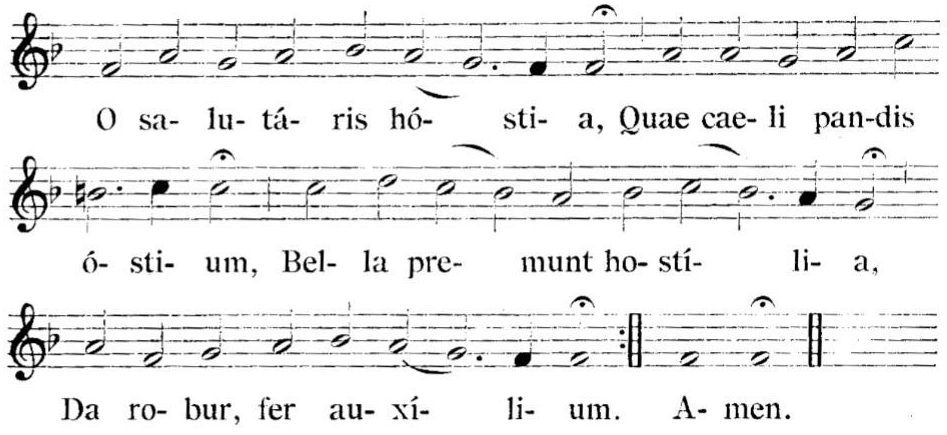
\includegraphics[width=\linewidth]{../ordinaires/o-salutaris.jpg}
  \end{figure}

  \begin{center}
    \begin{footnotesize}
      \textit{
        Ô réconfortante
        Hostie, Qui nous
        ouvres les portes du
        ciel, les armées ennemies
        nous poursuivent,
        Donne-nous la force,
        porte-nous secours.
      }
    \end{footnotesize}
  \end{center}

  \begin{multicols}{2}
    \parindent=0pt
    \begin{flushright}
      O vere digna Hostia,\\
      Spes unica fidelium,\\
      In te confidit Francia,\\
      Da pacem, serva lilium.\\
    \end{flushright}
    \columnbreak
    \textit{
      Ô vraiment digne Hostie,\\
      Unique espoir des fidèles,\\
      en toi se confie la France,\\
      Donne-lui la paix, conserve le lys.\\
    }
  \end{multicols}
  \begin{multicols}{2}
    \begin{flushright}
      Uni trinoque Domino\\
      Sit sempiterna gloria :\\
      Qui vitam sine termino,\\
      Nobis donet in patria. Amen.\\
    \end{flushright}
    \columnbreak
    \textit{
      Au Seigneur unique en trois personnes,\\
      La gloire éternelle;\\
      qu'il nous donne en son Royaume\\
      La vie qui n'aura pas de fin. Amen\\
    }
  \end{multicols}

  \begin{center}
    \rule{2cm}{0.4pt}
  \end{center}

  \newpage

  % \begin{center}
  %   \textcolor{red}{\normalsize{Antienne à la Sainte Vierge.}}\\
  % \end{center}
  \begin{center}
    \textcolor{red}{\large{Salve Regína}}\\
    \begin{footnotesize}
      \textit{
      Du Dimanche de Pâques jusqu'au Vendredi après la Pentecôte inclusivement.
      }
    \end{footnotesize}
  \end{center}

  \gresetinitiallines{1}
  \greillumination{\initfamily\fontsize{11mm}{11mm}\selectfont S}
  \gregorioscore{an--salve_regina--solesmes}
  \medskip
  \begin{footnotesize}
    \textit{
      Salut, ô Reine, Mère de Miséricorde, notre vie, notre douceur, et notre espérance, salut. Vers vous nous élevons nos cris, pauvres exilés, malheureux enfants d'Eve. Vers vous nous soupirons, gémissant et pleurant dans cette vallée de larmes. De grâce donc, ô notre Avocate, tournez vers nous vos regards miséricordieux. Et, après cet exil, montrez-nous Jésus, le fruit béni de vos entrailles. Ô clémente, ô miséricordieuse, ô douce Vierge Marie.  
    }
  \end{footnotesize}

  \begin{multicols}{2}
    \parindent=0pt
    \begin{flushright}
      \textcolor{red}{\Vbar.} Ora pro nobis, Sancta Dei Génitrix.\\
      \textcolor{red}{\Rbar.} Ut digni efficiamur promissionibus Christi.\\
    \end{flushright}

    \columnbreak
    
    \textit{\textcolor{red}{\Vbar.} Priez pour nous, Sainte Mère de Dieu. \\
    \textcolor{red}{\Rbar.} Afin que nous soyons rendus dignes des promesses du Christ.}\\
  \end{multicols}

  \begin{multicols}{2}
    \parindent=0pt
    Omnípotens sempitérne Deus, qui gloriósæ Vírginis Matris Maríæ corpus et ánimam, ut dignum Fílii tui habitáculum effici mererétur, Spíritu Sancto cooperánte, præparásti : \textcolor{red}{†} da, ut, cujus commemoratióne lætámur, \textcolor{red}{*} ejus pia intercessióne, ab instántibus malis et a morte perpétua líberémur.\\ Per eúmdem Christum Dóminum nostrum.\\ 
    \textcolor{red}{\Rbar.} Amen.

    \columnbreak

    \textit{Dieu tout-puissant et éternel, qui avez préparé le corps et l’âme de la glorieuse Vierge et Mère Marie afin d’en faire une demeure digne de votre Fils, avec le concours du Saint-Esprit ; faites que, par la prière maternelle de celle dont nous évoquons avec joie la mémoire, nous soyons affranchis du mal présent et de la mort éternelle.\\
    Amen.
    }
  \end{multicols}

  \begin{center}
    \rule{2cm}{0.4pt}
  \end{center}

  \newpage

  \begin{center}
    \textcolor{red}{\large{En l'honneur Du Saint Sacrement}}
  \end{center}

  \gresetinitiallines{1}
  \greillumination{\initfamily\fontsize{11mm}{11mm}\selectfont T}
  \gregorioscore{../ordinaires/hy--tantum_ergo--solesmes}

  \begin{center}
    \begin{footnotesize}
      \begin{enumerate}[label=\textcolor{red}{\emph{\arabic*}}]
        \item \textit{Devant un sacrement si grand, prosternons-nous, adorons ; et que les symboles anciens s'effacent devant le rite nouveau ; que la foi vienne suppléer à la faiblesse de nos sens.}
        \item \textit{Au Père et au Fils louanges et acclamations, gloire honneur et puissance ainsi que bénédictions. A Celui qui de tous deux procède offrons une égale louange.}
      \end{enumerate}
    \end{footnotesize}
  \end{center}

  \medskip

  \begin{multicols}{2}
    \parindent=0pt
    \textcolor{red}{\Vbar.} Panem de caelo praestitisti eis.\\
    \textcolor{red}{\Rbar.} Omne delectamentum in se habentem.\\
    
    \textit{\textcolor{red}{\Vbar.} Tu leur a donné le pain du ciel.\\
    \textcolor{red}{\Rbar.} Toute saveur se trouve en lui.}\\
    
  \end{multicols}

  \bigskip

  \begin{center}
    \textcolor{red}{\large{Oraison}}
  \end{center}

  \begin{multicols}{2}
    \parindent=0pt
    Deus, qui nobis sub sacramento mirabili
    passionis tuæ memoriam reliquisti : \textcolor{red}{~†}
    tribue, quæsumus, ita nos Corporis et
    Sanguinis tui sacra mysteria venerari, \textcolor{red}{~*} ut
    redemptionis tuæ fructum in nobis
    jugiter sentiamus.\\
    Qui vivis et regnas
    cum Deo Patre in unitate Spiritus Sancti,
    Deus, per omnia sæcula sæculorum.
    Amen.
    \columnbreak

    \textit{
      Seigneur Jésus Christ, dans cet admirable
      sacrement tu nous a laissé le mémorial de
      ta passion ; donne-nous de vénérer d’un si
      grand amour le mystère de ton Corps et de
      ton Sang, que nous puissions recueillir
      sans cesse le fruit de ta rédemption. Toi
      qui règnes avec le Père et le Saint Esprit
      pour les siècles des siècles.
      Amen. 
    }
  \end{multicols}

  \begin{center}
    \rule{2cm}{0.4pt}
  \end{center}

  \newpage


  \begin{center}
    \textcolor{red}{\large{Louanges divines}}
  \end{center}


  \begin{normalsize}
    \parindent=0pt
    Dieu soit béni.\\
    Béni soit son Saint Nom.\\
    Béni soit Jésus-Christ, vrai Dieu et vrai homme.\\
    Béni soit le Nom de Jésus.\\
    Béni soit son Sacré Cœur.\\
    Béni soit son précieux Sang.\\
    Béni soit Jésus dans le très Saint Sacrement de l’autel.\\
    Béni soit l’Esprit Saint Consolateur.\\
    Bénie soit l’auguste Mère de Dieu, la très Sainte Vierge Marie.\\
    Bénie soit sa Sainte et Immaculée Conception.\\
    Bénie soit sa glorieuse Assomption.\\
    Béni soit le nom de Marie, Vierge et Mère.\\
    Béni soit Saint Joseph, son très chaste époux.\\
    Béni soit Dieu dans ses anges et dans ses saints.\\
    Seigneur, donnez-nous des prêtres.\\
    Seigneur, donnez-nous de saints prêtres.\\
    Seigneur, donnez-nous beaucoup de saints prêtres.\\
    Seigneur, donnez-nous beaucoup de saintes vocations religieuses.\\
  \end{normalsize}


  % \newpage

  \begin{center}
    \textcolor{red}{\large{Déposition}}\\
    \textit{Psaume 116}
  \end{center}

  \gresetinitiallines{1}
  \greillumination{\initfamily\fontsize{11mm}{11mm}\selectfont L}
  \gregorioscore{../temps_pascal/psaumes/ps--laudate_dominum_omnes_gentes_(psalmus_116)--solesmes}
  \bigskip
  \begin{footnotesize}
    \textit{
      Louez le Seigneur, tous les
      peuples ;
      Fêtez-Le, tous les pays !
      Son Amour envers nous
      S'est montré le plus fort ;
      Eternelle est la Fidélité du
      Seigneur !
      Gloire au Père, au Fils
      Et au Saint-Esprit,
      Comme il était au
      commencement,
      Maintenant et toujours,
      Pour les siècles des siècles,
      amen.
    }
  \end{footnotesize}

\end{document}